\chapter{Introduction}
\begin{chapquote}{John Gage, \textit{slogan for Sun Microsystems}}
The network is the computer.
\end{chapquote}

Fourty years since John Gage has coined the catchy slogan for Sun Microsystems, networked computers are being used around the world more than ever, empowering a vast range of modern technologies that our societies are increasingly depending upon.  This directly corresponds to the ever increasing higher bandwidth and lower requirements \timos{what means lower requirements here?} of datacenter networks: 100 and 200 Gbps Ethernet and InfiniBand are becoming de-facto standards; link speeds of 400 Gbps and beyond are already being developed and deployed~\cite{miller_pursuit_nodate}.

On the other hand, CPU processing power have not been scaling up at the same pace with the increase of link speeds and the higher packet processing overhead that comes with these speeds.  \emph{Remote Direct Memory Access} (RDMA) is one of the many offloading technologies designed to reduce packet processing overheads on the CPU.  While the RDMA approach reduces network-related processing overheads, the actual consumption of the packet payload still happens on the CPU cores.  Modern CPU cores are built with complicated microarchitectures optimised for compute-heavy workloads instead of most packet-processing workloads that involve simple arithmetics and data movement.  The CPU cycles spent processing packets would be best utilised to perform the compute-heavy tasks instead, \timos{of which? check grammar} of which the device is designed for. \timos{I think this needs a figure/citations to show these trennds - idea is good though}

SmartNICs are a recent movement towards offloaded packet processing to free the CPU from packet processing and thus spend more time handling the typical computation tasks.  They come in different programming models and dataflow models.  Among different paradigms, \emph{streaming Processing in the Network} (sPIN)~\cite{hoefler_spin_2017} developed at ETH Z\"urich proposes a \emph{bump-in-the-wire} \timos{it feels like there is a sentence missing explaining sNIC styles} style network accelerator with a micro-architecture optimised for packet processing and fine-grain memory hierarchies and data movement acceleration.  It offers precise control to the programmers to build high-performance networked applications that are offloaded completely to the SmartNIC.

The sPIN paradigm has been evaluated extensively with diverse networked applications~\cite{di_girolamo_network-accelerated_2019, cao_accelerating_2022, di_girolamo_building_2022}, showcasing its capability of offloading complicated applications to a sPIN-based network accelerator.  Up to the writing of this thesis, however, all evaluations of sPIN took place in simulation and there lacked a real-world end-to-end demo on hardware.  While simulation works well to demonstrate capabilities of the paradigm in a \emph{synthetic} environment, an end-to-end evaluation involving all parts of the final system would uncover unforeseen design and implementation shortcomings and offer valuable insights to further improve the paradigm.

\begin{figure}
    \centering
    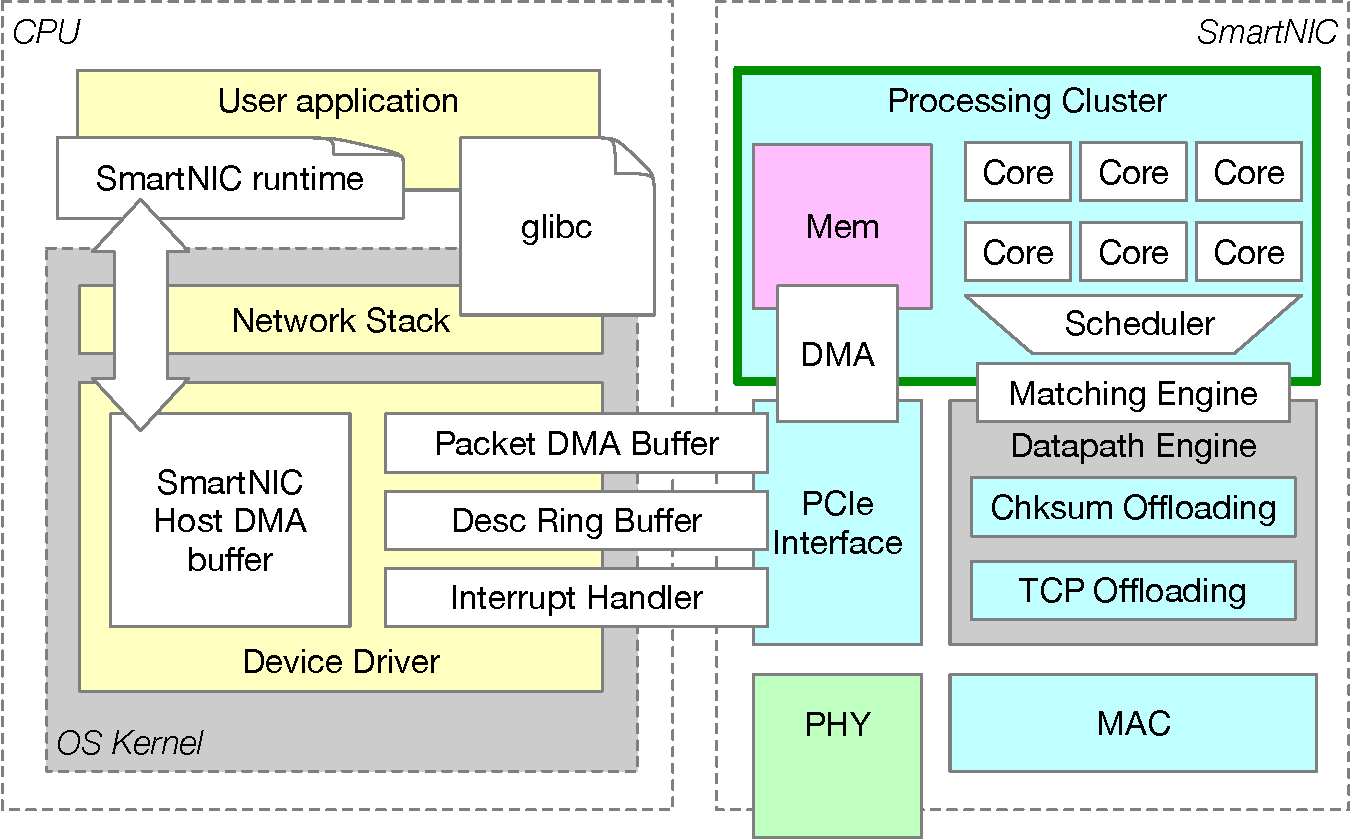
\includegraphics[width=.9\linewidth]{figures/system-overview.pdf}
    \caption{Overview of the complete server system, showing the software stack on the CPU and hardware components on the SmartNIC.  The green box marks the existing PsPIN processing cluster available from previous work.  Everything else needs to be developed, integrated and tested.}
    \pengcheng{update style to match background diagrams}
    \label{fig:full-system}
\end{figure}

\section{Contributions} \label{sec:contributions}

In this section of the introduction, we give a brief summary of the contributions of this thesis and references of where they are explained in the text.  An overview functional diagram of the system is shown in \Cref{fig:full-system}.

First of all, we built \emph{FPsPIN}, the first full-system demo of sPIN in hardware based on the PsPIN~\cite{di_girolamo_pspin_2021} implementation of sPIN and the Corundum~\cite{forencich_corundum_2020} open-source Ethernet \emph{network interface card} (NIC).  This allows fast testing of packet \emph{handlers} (code that runs on the sPIN cluster, more details in \Cref{sec:background-spin}) in comparison to the slow cycle-accurate simulator (\Cref{sec:background-pspin}).  The hardware (\Cref{chap:hardware}) and software (\Cref{chap:software}) components bridge the missing parts in the PsPIN prototype to allow sending and receiving of packet data from real NICs and, most importantly, completes the \emph{host-side} programming model of sPIN.  This allows development of complete sPIN applications with both the NIC-side handlers and host-side application.  In all, the demo system greatly facilitates development both of the sPIN platform as well as applications designed for it.

An important yet largely unexplored benefit of sPIN is the possibility of \emph{computation/communication overlap} by offloading packet processing tasks to the SmartNIC.  We port the MPI Datatypes~\cite{ropo_processing_2009} sPIN handlers~\cite{di_girolamo_network-accelerated_2019} to the FPsPIN platform (\Cref{sec:mpi-datatypes-demo}) to demonstrate the ratio of overlapping between the computation and communication tasks, as well as interference from each other.  This demonstrates sPIN's potential of accelerating networked applications and improving effiency.

Last but not least, we discovered numerous shortcomings and points of improvement in the sPIN specification~\cite{hoefler_spin_2017} (\Cref{chap:spin-revisited}) during the development of the FPsPIN prototype system.  We discuss about the issues closely with the sPIN team and work together towards a more complete and sensible specification for other implementors of the paradigm.  Several of the proposed changes have already been incorporated back into the specification.